\documentclass[12pt]{beamer}

\usepackage{beamerthemeHannover, graphicx, clrscode, amsmath, amssymb, multicol}
\setbeamercolor{sidebar}{use=structure,bg=gray!20!green!60!white}

\title{Creating CPAN Modules with SWIG}
\author[J.A. Leto]{Jonathan Leto}
\date{}

\begin{document}
\frame{
    \titlepage
    \begin{center}
    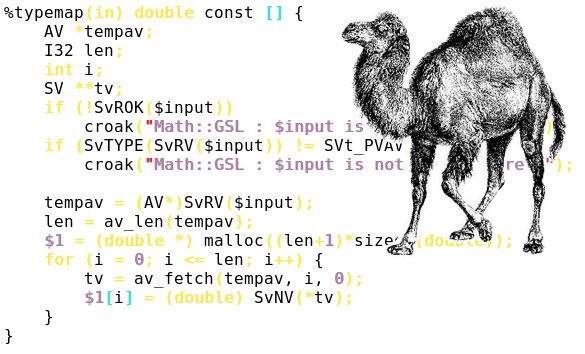
\includegraphics[width=5.84cm, height=3.85cm]{swig_camel}
    \end{center}
}

\section{Overview}

\frame{
    \frametitle{Overview}
    \begin{itemize}
        \item Philosophy
        \item Basics
        \item Definitions
        \item The Big Picture
        \item Motivation for Math::GSL
        \item History of Math::GSL
        \item Module::Build and SWIG
        \item Gotchas
    \end{itemize}
}
\section{Philosophy}
\frame{
    \frametitle{Don't Write Glue}
    \begin{columns}[t]
        \begin{column}{5cm}
            {\bf{XS = GLUE}}\\
        \end{column}
        \begin{column}{5cm}
            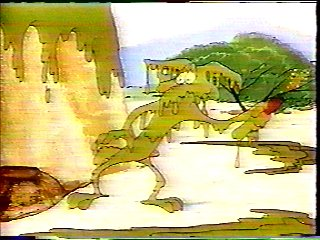
\includegraphics[width=5.00cm, height=5.00cm]{acmeglue}
        \end{column}
    \end{columns}

}

\section{Basics}
\subsection{Intro to SWIG}
\frame{
    \frametitle{What is SWIG?}
    \begin{itemize}
        \item Simplified Wrapper Interface Generator
        \item Creates a scripting language API to a C/C++ library 
        \item 18 target languages supported
        \item Reads header files and transforms datatypes between languages
    \end{itemize}
}
\frame{
    \frametitle{SWIG Example Code}
}
%		\begin{center}
%	\includegraphics[width=10cm,bb=0 0 1530 666]{ocb1.png}
% ocb1.png: 72dpi, width=40.96cm, height=19.90cm, bb=0 0 1161 564
%	\end{center}

\frame{
    \frametitle{Active Development Continues}

    \begin{itemize}
    \item Scientific Computing applications built on top of Math::GSL
    \item foo
    \end{itemize}
}

\frame{
    \frametitle{Thanks}

    \begin{itemize}
        \item Eric Wilhelm
        \item \#pdx.pm
        \item Leslie Hawthorn and the Google Summer of Code crew
    \end{itemize}
}

\end{document}
